\chapter{Entropy production in continuous phase space systems}
\label{chap:flow}

The contents of this chapter are again an in-depth description of a publication, this time in the Journal of Statistical Physics, under the same title \cite{flow-paper}.

An overview is as follows: The first section will talk about how to transfer some of the ideas used in the previous chapter to a continuous setting, and what problems arise on the way there. Afterwards, in section~\RefSection{sec:sde}, a brief overview over stochastic differential equations (SDEs) is given, before the main model of interest is introduced in section~\RefSection{sec:underdamped-model}. Section~\RefSection{sec:differential entropy production}, the chapter's main part, will then develop a new entropy definition, and compare it with a previously known one in the process.

The most important result will be that the production of environmental entropy is in a certain sense ambiguous, allowing multiple different definitions that all agree in their end results.


%%%%%%%%%%%%%%%%%%%%%%%%%%%%%%%%%%%%%%%%%%%%%%%%%%%%%%%%%%%%%%%%%%%%%%%%%%%%%%
\section{From discrete to continuous systems}
\label{sec:discrete to continuous}
%%%%%%%%%%%%%%%%%%%%%%%%%%%%%%%%%%%%%%%%%%%%%%%%%%%%%%%%%%%%%%%%%%%%%%%%%%%%%%

The basis of Chapter~\ref{chap:thingie} was the assumption of a discrete system \(\Omega = \{c_1, c_2, \ldots\}\). On the other hand, many processes occurring in nature are not discrete. This chapter describes an attempt to transfer the concept of environmental entropy used before to a continuous phase space system governed by Hamiltonian equations of motion.

Recall that a Markov process is fully described by an initial configuration \(p^\init\) and a set of transition rates \(w\), which provide a way of getting from one state to the next. Conceptually, this can be continualized to the case where the configuration is the location of a particle, leading to a system described by
%
\begin{equation}
	\label{eqn:overdamped}
	\dot q(t) = f(q,t) + g(q,t)\xi(t) ~,
\end{equation}
%
which can be understood in two different ways. Coming from a Markov process, \(f\) corresponds to the bias of the transition rates to go towards a certain state, and \(g\) accounts for how the noise depends on location. On the other hand, seen from a neutral standpoint, \(f\) is of course a force term, and \(g\xi\) is the randomness of the system due to a heat bath represented by Gaussian noise \(\xi(t)\), for example.

Most noticably, the above equation does not include any form of momentum. This can be seen as a residue of the Markov property, which was previously informally described as ``momentum-less''; in a continuous differential equation (DE), this description is much more meaningful, because very high damping gets rid of any momentum right away. For this reason, equations of the form \RefEqn{eqn:overdamped} are called \emph{overdamped}, and could for example describe the motion of a bacteria in water (which happens to be quite thick for small organisms \cite{sengupta}. Many of the quantities associated with Markov processes have clear corresponding quantities in the overdamped case, in particular the notion of a ``jump'' from one state to the other has a reverse, allowing the definition of environmental entropy to carry over quite directly \cite{seifert-overdamped},
%
\begin{equation}
	\Delta\SEnv = \ln\frac{p[\gamma | q_0]}{p^\dagger[\gamma^\dagger | q_0^\dagger]}
\end{equation}
%
where \(p[\gamma]\) is the probability of taking the forward path \(\gamma\), and \(p^\dagger[\gamma^\dagger]\) is the likelihood of walking that same path in reverse direction. The \(\dagger\) (``dagger'') or \emph{conjugation} operation encodes this reversal in the obvious way: for a process running from time \(t=0\) to \(T\),
%
\begin{equation}
	\begin{split}
		q^\dagger(t) &= q(T-t) \\
		q_0^\dagger(t) &= q_T \\
		t &\overset\dagger\rightarrow T-t
	\end{split}
\end{equation}
%
where the last line is important if the coefficients in \RefEqn{eqn:overdamped} have an explicit time dependency. Note that the \(\dagger\) operation is \emph{not reversing time}, it only stands for walking the same path in reverse directions, probably better described as ``making the same decisions, but in reverse order''. Figure~\RefFigure{fig:knight continuous} also illustrates this process.

\begin{figure}[htbp]
	\centering
	\begin{tikzpicture}[
		move1/.style={red, thick},
		move2/.style={blue, thick}
		]

	\draw[step=1cm, gray, shift={(0.5,0.5)}] (-3.2,-1.2) grid (2.2,3.2);


	\begin{scope}
		\newcommand\LineWidth{2}
		\draw[move1, line width=\LineWidth, postaction={decorate},
				decoration={
					markings,
					mark=at position .2 with {\arrow{left to};},
					mark=at position .4 with {\arrow{left to};},
					mark=at position .6 with {\arrow{left to};},
					mark=at position .8 with {\arrow{left to};}
				}
			]
			plot[smooth,tension=0.7] coordinates{(0,0) (2,1) (1,3) (0,1) (-2, 2)};
		\draw[move2, line width=\LineWidth, postaction={decorate},
				decoration={
					markings,
					mark=at position .25 with {\arrowreversed{right to};},
					mark=at position .45 with {\arrowreversed{right to};},
					mark=at position .65 with {\arrowreversed{right to};},
					mark=at position .85 with {\arrowreversed{right to};}
				}
			]
			plot[smooth,tension=0.7] coordinates{(0,0-0.075) (2+0.075,1) (1,3+0.075) (0,1+0.075) (-2, 2+0.075)};
	\end{scope}


	\newcommand\smallR{0.075}
	\newcommand\Move[3]{
		\draw[->, #3, shorten >= \smallR cm, shorten <= \smallR cm] #1 -- #2;
		\draw[#3] #2 circle (\smallR);
	}
	
	\node[move1] at (-1,0.9) { \(\gamma\) };
	\node[move2] at (0,1.8) { \(\gamma^\dagger\) };

	\draw[yellow, fill=white, thick] (-2,2) circle (0.4);
	\node[yellow] at (-2,2) { \(x_0^\dagger\) };

	\draw[color=yellow, fill=white, thick] (0,0) circle (0.4);
	\node[yellow] at (0,0) { \(x_0\) };

\end{tikzpicture}
	\caption[]{
		The knight from figure~\RefFigure{fig:knight}, but now in a continuous setting, where the configuration is \((x,y)\in\Set R^2\). The {\color{red}forward path \(\gamma\)} is taken with probability \(p[{\color{red}\gamma}|{\color{yellow}x_0}]\), and the {\color{blue}backward/conjugate path \(\gamma^\dagger\)} occurs with probability \(p^\dagger[{\color{blue}\gamma^\dagger}|{\color{yellow}x_0^\dagger}]\). In both cases, the paths can be constructed so time runs forward as the particle follows the trajectory.
	}
	\label{fig:knight continuous}
\end{figure}

Of course not all systems in nature are overdamped in the continuous case, just like not every discrete system has the Markov property. These non-overdamped -- \emph{underdamped} -- systems take the full Hamiltonian phase space into account, and the Hamiltonian equations of motion take the form
%
\begin{equation}\begin{split}
	\label{eqn:general hamiltonian equations}
	\dot q(t) &= f_q(q,p,t) + g_q(q,p,t)\xi_q(t) \\
	\dot p(t) &= f_p(q,p,t) + g_p(q,p,t)\xi_p(t)
\end{split}\end{equation}
%
As will be discussed later, it is nontrivial to introduce the concept of environmental entropy production in this scenario. The key reason to this is that a path cannot be reversed in a straight-forward way (i.e. the ``\(\dagger\)'' operation is not easily defined), and the main result of this chapter is a new way this path reversal can be defined, and what the consequences are.

To explain this, consider simply carrying over the \(\dagger\)~operation from the above (overdamped) case. The stochastic trajectory, now through \((q,p)\) space, will be transformed \`a la
%
\begin{equation}\begin{split}
	\gamma &= \Bigl\{\bigl(q(t),p(t)\bigr)\Bigr\}
	\\ \overset\dagger\longrightarrow \quad
	\gamma^{\dagger_\text{na\"ive}}
		&= \Bigl\{\bigl(q^{\dagger_\text{na\"ive}}(t),p^{\dagger_\text{na\"ive}}(t)\bigr)\Bigr\}
		= \Bigl\{\bigl(q(T-t),p(T-t)\bigr)\Bigr\}
\end{split}\end{equation}
%
but it turns out that the velocity \(\dot q\) has a different sign as momentum \(p\) in this definition, leading to an unphysical path.







%%%%%%%%%%%%%%%%%%%%%%%%%%%%%%%%%%%%%%%%%%%%%%%%%%%%%%%%%%%%%%%%%%%%%%%%%%%%%%
\section{Stochastic differential equations}
\label{sec:sde}
%%%%%%%%%%%%%%%%%%%%%%%%%%%%%%%%%%%%%%%%%%%%%%%%%%%%%%%%%%%%%%%%%%%%%%%%%%%%%%

There are multiple equivalent approaches to stochastic differential equations (SDEs), i.e. differential equations with a probabilistic or ``noise'' term. There are two important distinctions to make between the three commonly used ones.

The goal of this section is not providing an introduction to SDEs, but to illustrate different formalisms briefly, and mention their key concepts. A more rigorous yet practical treatment of stochastic calculus can be found in e.g. \cite{sde}, which also served as a main source for what follows.


%%%%%%%%%%%%%%%%%%%%%%%%%%%%%%%%%%%%%%%%%%%%%%%%%%%%%%%%%%%%%%%%%%%%%%%%%%%%%%
\subsection{Math vs. physics}
\label{sec:math vs physics}
%%%%%%%%%%%%%%%%%%%%%%%%%%%%%%%%%%%%%%%%%%%%%%%%%%%%%%%%%%%%%%%%%%%%%%%%%%%%%%

The area usually associated with stochastic differential equations in mathematics is \Ito{} calculus, while its close relative named after Stratonovich is what physics typically deals with. Both of these deal with equations of the form
%
\begin{equation}
	\label{eqn:sde}
	\d X_t = f(X_t,t) \d t + g(X_t,t) \d W_t
\end{equation}
%
describing how a \emph{microscopic} quantity \(X\) evolves under the influence of a deterministic drive \(f\) and a stochastic contribution \(g\,\d W_t\), where \(\d W_t\) is the Wiener measure accounting for the stochasticity. The Weiner process is the fundamental building block in SDEs; \(W_t\) can be interpreted as the position of a random walk at time \(t\), and \(\d W_t\) is a ``small'' increase of this random walk as time advances a little. The solution of such a SDE will be a probability distribution for the value of \(X\).
Informally -- but maybe more intuitive -- the above equation is ``divided by \(\d t\)'' to yield
%
\begin{equation}
	\dot X(t) = f(X(t),t) + g(X(t),t)\frac{\d W_t}{\d t} ~,
\end{equation}
%
called a Langevin equation, and \(\d W_t(t)/\d t\) can be interpreted as Gaussian noise \(\xi(t)\),
\begin{equation}
	\dot X(t) = f(X(t),t) + g(X(t),t)\xi(t)~.
\end{equation}
%
This is the form often used in physics. In this setting, the noise is usually defined by its statistical properties, most commonly
\begin{align}
	\langle\xi(t)\rangle &= 0 \\
	\langle\xi(t)\xi(t')\rangle &\propto \delta(t-t')
\end{align}
%
and can therefore be pictured as a quantity fluctuating around \(0\) so wildly that there are no correlations between any given different points in time. The advantage of this approach of course is that \(\xi\) can be treated as an ordinary function with certain special properties.


%%%%%%%%%%%%%%%%%%%%%%%%%%%%%%%%%%%%%%%%%%%%%%%%%%%%%%%%%%%%%%%%%%%%%%%%%%%%%%
\subsection{\Ito{} vs. Stratonovich}
\label{sec:ito-stratonovich dilemma}
%%%%%%%%%%%%%%%%%%%%%%%%%%%%%%%%%%%%%%%%%%%%%%%%%%%%%%%%%%%%%%%%%%%%%%%%%%%%%%

There is a surprising difference between the \Ito{} and Stratonovich schemata used to describe a system's behaviour. Suppose one wanted to solve a SDE numerically. The naive approach would take the current state of the system \(X(t)\), and extrapolate its new value using the SDE (using a suitably generated random number \(\Cal R\) for the noise) a timespan \(\d t\) later \`a la
%
\begin{equation}
	X(t+\d t) = f(X(t))\d t + g(X(t)) \Cal R ~.
\end{equation}
%
However, this leaves one question open: why should the functions be evaluated at the starting point of the interval \([t,t+\d t]\), and not for example at \(t_\text{eval} = t+\d t/2\)? And indeed it turns out that the result depends on the choice of this evaluation point. In other words, there is an ambiguity in solving SDEs: all of the schemata
%
\begin{align}
	X(t+\d t) &= f(X(t+a\,\d t))\d t + g(X(t+a\,\d t)) \Cal R \\
	a &\in [0,1]
\end{align}
%
are theoretically valid ways of defining the integration of \RefEqn{eqn:sde}. Which value of \(a\) to choose depends on a number of factors, a couple of which are:
%
\begin{itemize}
	\item \emph{Modelling.} What is the nature of the noise? In finance, the randomness of the market is assumed to be a result of the current state and appears random due to the fact people are unpredictable. This is what the \Ito{} method models by setting \(a = 0\). On the other hand, for example in physics or biology, the noise often originates from a second, underlying and inaccessible process, such as temperature-related fluctuations, and setting \(a = 1/2\) (=~Stratonovich) accounts for this independence of noise and system by not preferring either side of the timestep over the other. Other values of \(a\) are not commonly used, although they do appear in special cases \TODO{ref: jaegon mentioned \(a=1\)}.
	\item \emph{Pragmatism.} Some formulas are easier in certain formulations. A good example is the chain rule, which is called just that in the Stratonovich case, whereas its analogon has the telling name ``\Ito{}'s lemma''.
\end{itemize}
%
In the context of these issues, it is important to mention that both approaches are equvalent and can be converted into each other via
%
\begin{equation}
	\int_0^Tf(W_t,t)\circ\d W_t
	=
	\int_0^Tf(W_t,t)\,\d W_t
	+
	\frac12\int_0^T \partial_xf(W_t,t)\,\d t ~,
\end{equation}
%
where the convention is that ``\(\circ\,\d W_t\)'' stands for Stratonovich integration, and anything without special syntax is \Ito{}. The spatial derivative \(\partial_x\) is to be read as with respect to \(f\)'s first argument (which appears with explicit mention of the Wiener process in the integrands). As can be seen above, both approaches are identical if the integrand \(f\) is spatially constant; otherwise, the nonvanishing integral will be referred to as a \emph{drift term}.


%%%%%%%%%%%%%%%%%%%%%%%%%%%%%%%%%%%%%%%%%%%%%%%%%%%%%%%%%%%%%%%%%%%%%%%%%%%%%%
\subsection{Micro vs. macro}
\label{sec:fp introduction}
%%%%%%%%%%%%%%%%%%%%%%%%%%%%%%%%%%%%%%%%%%%%%%%%%%%%%%%%%%%%%%%%%%%%%%%%%%%%%%

SDEs like eq.~\RefEqn{eqn:sde} assume a single quantity \(X\), tracks its behaviour over time, and accumulates this in a final probability distribution for its value. This is a microscopic approach, effectively equivalent to repeating the same experiment with identical initial conditions (i.e. particle in the same place) many times, recording each individual result, and putting that in a histogram.

However, individual partcles are rarely\footnote{For a case where this \emph{is} possible, consider biophysical models of individual cells, or the Brownian motion of small particles in liquid \cite{sengupta}.} accessible, and the starting point of the experiment is a probability distribution in the first place. This scenario is described by the Fokker-Planck (FP) equation, which can be interpreted as a generalized Heat Equation:
%
\begin{equation}
	\label{eqn:fp}
	\begin{split}
	\partial_tP(x,t)
	&= - \partial_x (f(x,t)P(x,t)) + \partial_x^2 (D(x,t)P(x,t)) \\
	&= -\partial_xj(x,t)
	\end{split}
\end{equation}
%
Like the Heat Equation, the FP equation describes a flow in terms of a current, just that this current can be more complex. Nevertheless, it still describes the evolution of an entire distribution over time, and not of one of its constituents. It can be shown that the FP equation is an alternative and equivalent formulation of the SDE
%
\begin{align}
	\d X_t = f(X_t,t)\d t + \sqrt{2 D(X_t,t)}\,\d W_t ~.
\end{align}
%
when integrated according to the \Ito{} calculus \cite{sde}.




%%%%%%%%%%%%%%%%%%%%%%%%%%%%%%%%%%%%%%%%%%%%%%%%%%%%%%%%%%%%%%%%%%%%%%%%%%%%%%
\section{Underdamped particle with additive noise}
\label{sec:underdamped-model}
%%%%%%%%%%%%%%%%%%%%%%%%%%%%%%%%%%%%%%%%%%%%%%%%%%%%%%%%%%%%%%%%%%%%%%%%%%%%%%

The treatment of the most general case of Hamiltonian motion, as stated for a single particle in \RefEqn{eqn:general hamiltonian equations}, turns out to be very complicated. For this reason, the model used here is a special case of said equations. That is not to say it is impractical though; many of the basic systems of classical mechanics can be described by these equations:
%
\begin{equation}\boxed{\begin{split}
	\label{eqn:model hamiltonian eqns of motion}
	\dot q &= p \\
	\dot p &= -V'(q) - \mu(p)p + \Gamma(p)\xi(t)
\end{split}}\end{equation}
%
This models a single one-dimentional particle of unit mass in full phase space \((q,p)\) subject to a conservative force field \(-V'(q)\), momentum-dependent friction \(\mu(p)\) and multiplicative noise \(\Gamma(p)\xi(t)\), where \(\xi(t)\) is Gaussian noise, implicitly defined via
%
\begin{equation}\begin{split}
	\langle\xi(t)\rangle &= 0 \\
	\langle\xi(t)\xi(t')\rangle &= 2D\delta(t-t')
\end{split}\end{equation}
%
and \(D\) is a diffusive coefficient.

The main question this chapter is trying to answer is what mechanism leads to the production of environmental entropy in a system that follows the above dynamics. In the sense of classical thermodynamics, environmental entropy can be thought of as the flow of energy in the form of heat in and out of a system (held at constant temperature). In the specific case here, the noise \(\xi\) adds energy to the system (decreasing the entropy in the environment due to the resulting cooling), while the friction takes out heat (increasing the entropy in the environment). Equipped with this simple knowledge of classical thermodynamics, it is already possible to formulate a definition for environmental entropy for a special case of the present model, namely if the particle is in equilibrium with a heat bath of temperature \(T\),
%
\begin{equation} T\d\SEnv = -\d Q \end{equation}
%
where \(Q\) is the heat contained in the system, and \(\SEnv\) is the environment's entropy. Since heat flowing from the environment into the system increases its entropy by \(\d\SEnv\) while decreasing the heat of the environment by \(\d Q\), a negative sign appears in the equation. Due to conservation of energy (first law of thermodynamics in the absence of mechanical work), the heat flow is precisely the energy flow between the systems, \(\d Q = \d E\), and \(E\) is simply the particle's energy,
%
\begin{equation} E = \frac{p^2}2 + V(q) \end{equation}
%
allowing the entropy production \(\d\SEnv\) to be written as
%
\begin{align}
	\d\SEnv(q,p) &= -\beta\,\d\left(\frac{p^2}2 + V(q)\right) \notag \\
	\Rightarrow \d\SEnv(q,p) &= -\beta p\d p - \beta V'(q)\d q ~.
	\label{eqn:classical environmental entropy production}
\end{align}
%
Reproducing this result from a microscopic approach however is nontrivial, and poses a strong consistency check for any theory trying to explain environmental entropy production in a similar setting. It will later turn out that under certain circumstances, some \emph{correct} theories fail to do so, yet yield correct physical results after another calculation. The reason and significance of this will be discussed at that point, where the terminology and formalism to deal with location-dependent ``thermodynamic'' quantities, like \(\d\SEnv(q,p)\) above, has been developed.






%%%%%%%%%%%%%%%%%%%%%%%%%%%%%%%%%%%%%%%%%%%%%%%%%%%%%%%%%%%%%%%%%%%%%%%%%%%%%%
\subsection{Fokker-Planck equation}
%%%%%%%%%%%%%%%%%%%%%%%%%%%%%%%%%%%%%%%%%%%%%%%%%%%%%%%%%%%%%%%%%%%%%%%%%%%%%%

A key quantity later will be the propagator of the Fokker-Planck equation, which can be seen as the continuous analogon of the Master quation \RefEqn{eqn:master}. For this reason, \RefEqn{eqn:model hamiltonian eqns of motion} has to be transformed into Fokker-Planck form. This will be done following the notation of \cite{sf} and defining phase space coordinates \(\vec x = (q,p)\), allowing it to be written as
%
\begin{equation}
	\d x_i = A_i(\vec x,t)\d t + B_i(\vec x, t)\d W_i
\end{equation}
%
where, as introduced in section~\ref{sec:math vs physics}, \(\d W_i\) can be interpreted as the random walk generated by the noise \(\xi(t)\).

The FP equation introduced in \ref{sec:fp introduction} was just concerned with a single dimension. In the present two-dimensional space (with coordinates \(\vec x\)), that equation has to be modified to
%
\begin{align}
	\label{eqn:fp phase}
	\partial_tP(\vec x,t)
	&= - \sum_{i=q,p} \partial_{x_i} (f_i(\vec x,t)P(\vec x,t)) + \partial_{x_i}^2 (D_i(\vec x,t)P(\vec x,t)) \\
	&= - \sum_{i=q,p} \partial_{x_i}j_i(\vec x,t)
\end{align}
%
taking into account the individual fluctuations each component of \(\vec x\) may be subject to. The coefficients are related to the above Langevin equation via
%
\begin{align}
	f_i(\vec x,t) &= A_i(\vec x,t) \\
	D_i(\vec x,t) &= \frac12B_i(\vec x,t)^2
\end{align}
%
when integrating accoring to \Ito{} scheme, done so for pragmatic reasons (there will be plenty of probably more interesting ambiguities later).
The FP equation corresponding to \RefEqn{eqn:model hamiltonian eqns of motion} there turns out to be
%
\begin{equation}\begin{split}
	\partial_t P(q,p,t) &= \Cal L \, P(q,p,t) \\
	\Cal L &= \mu(p)+p\mu'(p) + \Gamma(p)\Gamma''(p) + \Gamma'(p)^2 \\
	&\qquad +\bigl(p\mu(p) + 2\Gamma(p)\Gamma'(p) + V'(q)\bigr)\partial_p \\
	&\qquad +\frac12\Gamma(p)^2\partial_p^2 - p\partial_q ~.
\end{split}\end{equation}






%%%%%%%%%%%%%%%%%%%%%%%%%%%%%%%%%%%%%%%%%%%%%%%%%%%%%%%%%%%%%%%%%%%%%%%%%%%%%%
\subsection{Detailed balance redux}
%%%%%%%%%%%%%%%%%%%%%%%%%%%%%%%%%%%%%%%%%%%%%%%%%%%%%%%%%%%%%%%%%%%%%%%%%%%%%%

The idea of detailed balance (section \RefSection{sec:detailed balance}) is also applicable to continuous system, where as mentioned the Fokker-Planck equation \RefEqn{eqn:fp} takes over for the Master equation \RefEqn{eqn:master}. Analogous, a stationary FP equation means all macroscopic state variables are constant; in the present context it is of particular interest that no heat or environmental entropy is exchanged with the bath.

This can probably be better understood than in the discrete scenario even, where the explanation was quite abstract (``probability currents cancel out''). Eqns. \RefEqn{eqn:model hamiltonian eqns of motion} contains a friction term responsible for heating up the environment as the system moves, and also a noise term transferring energy (also in the form of heat) into the system. If these two contributions cancel out just right, then all that's left is a Hamiltonian system of a free particle in a potential, which is of course reversible and does not produce any heat.

Being in detailed balance introduces a connection between the friction terms \(\mu(p)\) and the noise coefficient \(\Gamma(p)\) in \RefEqn{eqn:model hamiltonian eqns of motion}. This relation can be obtainex explicitly by inserting a Boltzmann distribution (which is the equilibrium distribution of a system in thermal equilibrium with a heat bath) into the FP equation \RefEqn{eqn:fp phase} and setting it equal zero, namely
%
\begin{equation}
	P_\text{Boltz}(q,p)
	= \frac1Ze^{-\beta E(q,p)}
	= \frac1Z\exp\Bigl(-\beta \bigl(\tfrac{p^2}2+V(q)\bigr)\Bigr)
\end{equation}
%
The result is a first-order differential equation for \(\mu(p\)),
%
\begin{equation}\begin{split}
	0
	&=
	\frac12 \beta^2 p^2 \Gamma(p)^2
	- \beta p^2 \mu(p)
	- 2 \beta p \Gamma(p) \Gamma'(p)
	- \frac12 \beta  \Gamma(p)^2
	\\&\qquad
	+\Gamma(p) \Gamma''(p)
	+ \Gamma'(p)^2
	+ p \mu'(p)
	+ \mu(p)  ~.
\end{split}\end{equation}
%
Thanks to computer algebra systems\footnote{Mathematica~9.0.0.0}, the solution of this daunting equation is obtained quite easily, it is
%
\begin{equation}
	\mu(p) = \frac12\beta\Gamma(p)^2 - \frac1p\Gamma(p)\Gamma'(p) + C\frac1pe^{\frac{\beta p^2}2}
\end{equation}
%
where \(C\) is an arbitrary integration constant. However, since the last term is exponentially divergent for \(p\to\infty\), it unphysical: the mean acceleration of a system in equilibrium would be infinite. Therefore \(C = 0\) is the only suitable choice, and what remains is
%
\begin{equation}
	\label{eqn:einstein}
	\mu(p) = \frac12\beta\Gamma(p)^2 - \frac1p\Gamma(p)\Gamma'(p) ~.
\end{equation}
%
This generalizes the usual condition for detailed balance \(\mu = \frac12\beta\Gamma^2\) (also known as the Einstein relation) for momenum-independent (``additive'') noise and linear friction.



%%%%%%%%%%%%%%%%%%%%%%%%%%%%%%%%%%%%%%%%%%%%%%%%%%%%%%%%%%%%%%%%%%%%%%%%%%%%%%
\subsection{Short-time propagator}
%%%%%%%%%%%%%%%%%%%%%%%%%%%%%%%%%%%%%%%%%%%%%%%%%%%%%%%%%%%%%%%%%%%%%%%%%%%%%%

\subsubsection{General case}
\label{sec:general propagator case}

Like in the discrete case, a key ingredient to defining entropy production in a continuous setting is the notion of a path probability. This probability is given by the propagator or Green's function of the FP equation. It will be denoted \(G(\vec x'|\vec x;\,\Delta t)\), and can be read as the probability that a particle starting at phase space coordinates \(\vec x = (q,p)\) is found at a new point \(\vec x' = (q',p')\) at \(\Delta t\) time later. In the present work however, it will be sufficient to take the \emph{short-time} proagator into account, i.e. \(\Delta t\) is very small.

The short-time propagator \(G(\vec x'|\vec x;\,\d t)\) solves the FP equation to leading order in \(\d t\), and is therefore not uniquely defined:
%
\begin{enumerate}
	\item The short-time propagator need not be Gaussian, as long as the (``arbitrary-time'') macroscopic propagator is reproduced by it. According to the central limit theorem, any distribution with the correct first and second moments is sufficient. (Intuitively, this can be understood by the fact that many functions have identical first-order power series coefficients, but their actual global shape is influenced by the higher-order terms. In the present scenario, these terms are neglected, leading to said ambiguity.)
	%
	\item It is not clear where the fields contained in the FP equation \RefEqn{eqn:fp phase}, \(f_i(\vec x,t)\) and \(D_i(\vec x,t)\), have to be evaluated: at \(\vec x\), \(\vec x'\), between, somewhere in the neighbourhood? In general, an evaluation point at any \(\vec r = \varphi(\vec x,\vec x')\) with bijective \(\varphi\) will do \cite{wissel}. Conceptually, this is similar to the \Ito{}-Stratonovich dilemma introduced in the conext of stochastic differential equations in section~\RefSection{sec:ito-stratonovich dilemma}, but it is important to emphasize that this is a \emph{new, independent} ambiguity in addition to the previous one (which was resolved to integration according to \Ito{} scheme to obtain the FP equation from the SDE).
\end{enumerate}
%
To get a hold of the infinitely many short-time propagators, assume the evaluation point is linearly between the two end points,
%
\begin{equation}
	\vec r = (1-a)\vec x + a\vec x' \qquad a\in[0,1] ~,
\end{equation}
%
as done in \cite{sf}. Using \cite{wissel, donoso} this leads to the following expression for the propagator:
%
\begin{equation}\begin{split}
	\label{eqn:propagator general}
	G_a(\vec x'|\vec x;\,\d t)
	&= \prod_i \frac1{\sqrt{2\pi D_i\d t}}
	\\&\qquad
	\exp\left(
		- \frac{(\d x_i-A_i\d t+2aD_i'\d t)^2}{4D_i\d t}
		- a A_i'\d t
		+ a^2 D_i''\d t
		\right)
\end{split}\end{equation}
%
with the short-hands
%
\begin{align*}
	A_i &= A_i(\vec r,t)  &  A_i' &= \partial_{r_i}A_i(\vec r,t) \\
	D_i &= D_i(\vec r,t)  &  D_i' &= \partial_{r_i}D_i(\vec r,t)  &  D_i'' &= \partial_{r_i}^2D_i(\vec r,t) ~.
\end{align*}


\subsubsection{Applied to the model}

The system in question, \RefEqn{eqn:model hamiltonian eqns of motion}, consists of two coupled differential equations, but only one of them is stochastic, giving \(D_1\equiv0\). However, the propagator \RefEqn{eqn:propagator general} requires dividing by this quantity so it is not well-defined. For this reason, \RefEqn{eqn:model hamiltonian eqns of motion} is modified to add a ``very small'' (new, independent from \(\xi_p\)) noise term to the location, resulting in the system
%
\begin{equation}
	\label{eqn:underdamped sde epsilon}
	\begin{split}
		\dot q(t) &= p + \varepsilon \xi_q(t) \\
		\dot p(t) &= -V'(q) - \mu(p)p + \Gamma(p)\xi_p(t) ~;
	\end{split}
\end{equation}
%
the coefficient \(\varepsilon\) will later fall away on its own, justifying this rather ad-hoc addition.
The resulting propagator for this model then reads \TODO{check for correctness}
%
\begin{equation}
	\label{eqn:short time propagator}
	\begin{split}
		_\varepsilon G_a (q',p' | q,p;\,\d t)
		&= \frac1{2\pi\varepsilon\Gamma(r)\d t}
			\exp\Bigl(
				a^2(\Gamma(r)\Gamma''(r) + \Gamma'(r)^2)\d t
			\\&\quad
			-\frac{\bigl(V'(q+a\,\d q)\d t + 2 a\Gamma(r)\Gamma'(r)\d t + \d p + r\mu(r)\d t\bigr)^2}{2\Gamma(r)^2\d t}
			\\&\quad
			+ a\bigl(r\mu'(r)+\mu(r)\bigr)\d t
			- \frac{(\d q - r\d t)^2}{2\varepsilon^2\d t}
			\Bigr)
	\end{split}
\end{equation}
%
with
\begin{align*}
	\d q &= q' - q  &  \d p &= p' - p  &  r &= (1-a)p + ap' ~.
\end{align*}

As a consistency check, consider the limit \(\varepsilon\to0\). According to the differential equations above, this system should be deterministic in the position coordinate. And indeed the terms involving \(\varepsilon\) in \RefEqn{eqn:short time propagator} are of Gaussian shape, just like in the usual derivation of the \(\delta\)~distribution from a narrow Gaussian. More explicitly, the limit reads
%
\begin{equation}
	\label{eqn:delta-limit}
	\begin{split}
		G_a (q',p' | q,p;\,\d t) =
		\frac{\delta(\d q-r\d t)}{\sqrt{2\pi\d t}\Gamma(r)}\exp(\cdots)
	\end{split}
\end{equation}
%
where the \(\delta\) accounts for the deterministic location.



%%%%%%%%%%%%%%%%%%%%%%%%%%%%%%%%%%%%%%%%%%%%%%%%%%%%%%%%%%%%%%%%%%%%%%%%%%%%%%
\section{Differential entropy production}
\label{sec:differential entropy production}
%%%%%%%%%%%%%%%%%%%%%%%%%%%%%%%%%%%%%%%%%%%%%%%%%%%%%%%%%%%%%%%%%%%%%%%%%%%%%%

The focus of the main part of this chapter is the definition of differential environmental entropy \(\d\SEnv\). The term \emph{differential} will be used in multiple similar but different contexts; it can always be understood as some form of Taylor expansion of the finite entropy increase \(\Delta\SEnv\) in \(\d t\), \(\d q\) and \(\d p\) to lowest order. Which meaning is appropriate will be specified explicitly in ambiguous places.

The outline of what follows is this. First, an overview of Spinney and Ford's approach to defining \(\d\SEnv\) is given, which leads to the question what should be ``the state'' of an SDE. Inspired by this question, a new way of defining \(\d\SEnv\) will be proposed, and frequently compared to the other approach in the process of finding the corresponding formulas.



%%%%%%%%%%%%%%%%%%%%%%%%%%%%%%%%%%%%%%%%%%%%%%%%%%%%%%%%%%%%%%%%%%%%%%%%%%%%%%
\subsection{Spinney and Ford's entropy definition}
%%%%%%%%%%%%%%%%%%%%%%%%%%%%%%%%%%%%%%%%%%%%%%%%%%%%%%%%%%%%%%%%%%%%%%%%%%%%%%


In order to solve the issue of na\"ive path reversal mentioned in section~\RefSection{sec:discrete to continuous}, Spinney and Ford (SF) \cite{sf} choose to reverse time itself (\(t\to-t\)); more precisely, they take the time parity of all quantities into account, and mirror only those changing sign under time reversal. More explicitly, what they do is defining \(\dagger\) as \cite{sf-odd-even}
%
\begin{equation}\begin{split}
	\gamma &= \Bigl\{\bigl(q(t),p(t)\bigr)\Bigr\}
	\\ \overset\dagger\longrightarrow \quad
	\gamma^{\dagger_\SF}
		&= \Bigl\{\bigl(q^{\dagger_\SF}(t),p^{\dagger_\SF}(t)\bigr)\Bigr\}
		= \Bigl\{\bigl(\varepsilon q(T-t),\varepsilon p(T-t)\bigr)\Bigr\}
\end{split}\end{equation}
%
where \(\varepsilon\) is a parity operator, and equates to \(+1\) for even quantities such as \(q\) and \(-1\) for odd ones such as \(p\) under time reversal. Using this, they are able to use the entropy definition
%
\begin{equation}
	\Delta\SEnv = \ln\frac{p[\gamma | q_0]}{p^{\dagger_\SF}[\gamma^{\dagger_\SF} | q_0^{\dagger_\SF}]}
\end{equation}
%
to derive an expression for the differential environmental entropy production of arbitrary underdamped stochastic systems in full phase space \cite{sf}, given by
%
\begin{equation}
	\d\SEnv^\SF = \ln \frac{G_a(\vec x'|x;\,\d t)}{G_b(\vec x'^\dagger|\vec x^\dagger;\,\d t)} ~;
\end{equation}
%
recall that the propagator \(G_a(\vec x'|x;\,\d t)\) acorresponds to the probability to go from \(\vec x = (q,p)\) to \(\vec x'\) in the short time \(\d t\), plus an ambiguity parameter \(a\). In the case of the underdamped particle \RefEqn{eqn:underdamped sde epsilon} this then reads
%
\begin{equation}
	\label{eqn:DSEnv spinney main definition}
	\d\SEnv^\SF =
		\ln \frac
			{_\varepsilon G_a(q',p'|q,p;\,\d t)}
			{_\varepsilon G_b(q,-p|q',-p';\,\d t)} ~.
\end{equation}
%
A graphical representation of the paths constructed here can be found in the left part of figure~\RefFigure{fig:hf sf} (page~\pageref{fig:hf sf}).

In order to make this equation well-behaved in the limit of the ad-hoc parameter \(\varepsilon\to0\), both parts of the fraction have to peak at the same location; taking a step away from mathematics, this can be understood as the \(\delta\)~distributions in \RefEqn{eqn:delta-limit} cancelling. This leads to the condition \TODO{verify equation}
%
\begin{equation}
	(q'-q)-(p+a(p'-p))\d t = -\bigl((q-q') - (-p'+b(-p+p'))\d t\bigr)
\end{equation}
%
which is solved by \(b = 1 - a\), and therefore eliminates one of the propagator ambiguity parameters in \RefEqn{eqn:DSEnv spinney main definition}. SF obtain the same relation after a lengthy derivation in their appendix, and choose \(a = 0\) in the main text without further comment~\cite{sf}. Direct calculation of the entropy production results in the expression \TODO{verify}
%
\begin{equation}\begin{split}
	\label{eqn:sf entropy production}
	\d\SEnv^\SF
	&=\frac1{\Gamma^2}\bigl(
		- \mu\Gamma^2
		- \Gamma^3\Gamma''
		+ \Gamma^2\Gamma'^2
		- \Gamma^2p\mu'
	\\&\qquad\quad
		+ 2\mu\Gamma p\Gamma'
		- 2\mu pV'
		- 2 \Gamma\Gamma'V'
		\bigr) \d t
	\\&\qquad
		+\frac1{\Gamma^2}
		(-2\Gamma\Gamma' - 2\mu p) \d p
		+ \Cal O(\d t^2) +  \Cal O(\d p^3) ~;
\end{split}\end{equation}
%
where for the sake of brevity the explicit arguments of \(\Gamma(p)\), \(\mu(p)\) and \(V(q)\) have been dropped.
Note that the series expansion is to first order in \(\d t\) and \emph{second} order in \(\d p\).

This formula has some surprising properties. Most notably, in the case of a particle subject to linear friction (\(\mu(p) = \const\)) in detailed balance (\(\Gamma = \sqrt{2T\mu}\)) it reduces to
%
\begin{align}
	\d\SEnv^\SF = -\beta p \d p - \beta V'(q) \d q - \mu \d t
\end{align}
%
which has an additional term \(- \mu \d t\) compared to the textbook example \RefEqn{eqn:classical environmental entropy production}, indefinitely producing (negative) environmental entropy regardless of the state of the system -- take for example a resting free particle, \(p=0,V=\const\) to make this obvious -- when there should be no such production. This implausibility was in fact one of the motivations behind investigating the topic of continuous entropy further, although this specific issue was resolved upon further investigation (section \RefSection{sec:flow entropy}).

SF's approach has some further conceptually unsatisfactory properties though, first and foremost the \(\dagger\) operation is non-local in phase space: it maps \(p\to-p\), which may be in a completely different part of phase space where the Hamiltonian flow is not necessarily identical to the mirror image of the original flow. Furthermore, the start and end points of the normal trajectory are different from the ones for the conjugate process, which seems to be inconsistent with the idea behind the discrete environmental entropy production~\RefEqn{eqn:SEnv single jump definition}.

One last thing to mention here due to its later relevance is that the calculation to obtain \RefEqn{eqn:sf entropy production} can be done in the general case \(a = 1-b\) instead of setting \(a=0\) from the beginning on. The result is quite long and was therefore therefore moved appendix~\RefSection{sec:general SEnv expressions}, but for \(a = b = \frac12\) the resulting entropy reads
%
\begin{equation}\begin{split}
	\label{eqn:sf entropy production 1/2}
	\d\SEnv^{\SF_{1/2}} &=
	\frac1{\Gamma^2}\bigl(-2p\mu V'-2\Gamma\Gamma'V'\bigr)\d t
	+ \frac1{\Gamma^2}\bigl(-2p\mu-2\Gamma\Gamma'\bigr)\d p
	\\&\qquad
	+ \frac1{\Gamma^2}\bigl( -p\mu' + 2p\mu \tfrac{\Gamma'}\Gamma - \mu - \Gamma\Gamma'' + \Gamma'^2 \bigr) \d p^2
	\\&\qquad
	+ \Cal O(\d t^2) + \Cal O(\d p^3)
\end{split}\end{equation}
%
which is of course different from the \(a = 0\) result. Not very meaningful on its own, this term will reappear again in a different approach to entropy; the significance of this will become apparent later.




%%%%%%%%%%%%%%%%%%%%%%%%%%%%%%%%%%%%%%%%%%%%%%%%%%%%%%%%%%%%%%%%%%%%%%%%%%%%%%
\subsection{What is ``the state'' of a stochastic system?}
%%%%%%%%%%%%%%%%%%%%%%%%%%%%%%%%%%%%%%%%%%%%%%%%%%%%%%%%%%%%%%%%%%%%%%%%%%%%%%

The entropy definition, even in the continuous case, is based on the idea that environmental entropy is produced when the system changes from one state to another. SF's approach implicitly considers such a state to be the current location in phase space. As shown just above, this notion leads to strange results, illustrating an important difference between discrete and continuous settings: while randomness is the only source of dynamics in discrete models, continuous phase space systems consist of two parts: random \emph{and deterministic}.
When a continuous system changes ``its state'' in the previous sense, i.e. moves to a different point in phase space, this is not necessarily due to the noise, but could just be a consequence of deterministic processes, for example the ``SDE'' of the Hamiltonian model \RefEqn{eqn:model hamiltonian eqns of motion} with \(\mu \equiv \Gamma \equiv 0\), i.e. only the deterministic part of the system, seems to change state, but as it moves deterministically on the Hamiltonian flow it of course produces no entropy.

This realization leads to the question whether ``the state'' of a stochastic system is maybe something different, and not just the current location in phase space, and as will be shown in the following, an alternative definition can be made that solves these issues.

%%%%%%%%%%%%%%%%%%%%%%%%%%%%%%%%%%%%%%%%%%%%%%%%%%%%%%%%%%%%%%%%%%%%%%%%%%%%%%
\subsection{Hamiltonian orbit based entropy definition}
\label{sec:flow entropy}
%%%%%%%%%%%%%%%%%%%%%%%%%%%%%%%%%%%%%%%%%%%%%%%%%%%%%%%%%%%%%%%%%%%%%%%%%%%%%%

Reversible processes do not produce entropy, and any Hamiltonian process is reversible. A new definition of environmental entropy should satisfy this constraint, and therefore yield \(\Delta\SEnv = 0\) if a process follows a single Hamiltonian orbit; quite naturally, the idea that ``a state switch'' is a switch of such orbits, leading from one Hamiltonian process to another, lends itself as the basis for a new entropy definition, which will be developed in a moment. This approach will also have the side effect of eliminating the need to distinguish between odd and even variables, and yield a somewhat different expression for \(\Delta\SEnv\). However, it will turn out that the observables predicted by the new model lead to the \emph{same} expressions as SF's approach, indicating that there is a certain ambiguity in the way \(\Delta\SEnv\) cab be defined. The only necessary condition on the dynamics of the system for the following approach is that the equations of motion can be separated in Hamiltonian and non-Hamiltonian parts, so that the Hamiltonian orbits (i.e. the flow of the Hamiltonian part) can be identified.

More detailed, the new definition of the forward and backward paths is based on two Hamiltonian orbits \(\sigma\) and \(\sigma'\). The forward path \(\gamma\) is given in the same way as in SF's model, but the construction of the conjugate path -- denoted as \(\tilde\gamma\) instead of \(\gamma^\dagger\) to distinguish it from SF's approach -- is different, as illustrated in figure~\RefFigure{fig:hf sf} (page~\pageref{fig:hf sf}). The algorithm for the construction is as follows:
%
\begin{enumerate}
	\item The start point of the process is a phase space coordinate \(\vec x\), located on a Hamiltonian orbit \(\sigma\).
	\item The system evolves according to the full dynamics for a timespan \(\d t\), reaching a point \(\vec x'\) after following a trajectory \(\gamma\). \(\vec x'\) is located on some other Hamiltonian orbit \(\sigma'\).
	\item The weight of this path \(\gamma\) is given by the propagator \(G_a(\vec x'|\vec x;\,t,\d t)\).
	\item The starting point of the conjugate process \(\tilde{\vec x}'\) is reached by tracing back the Hamiltonian orbit through \(\vec x'\), \(\sigma'\), for a timespan \(\d t\).
	\item Similarly, the end point of the conjugate process \(\tilde{\vec x}\) is where the system would have gone from \(\vec x\), had it only followed the Hamiltonian orbit \(\sigma\) for a time \(\d t\).
	\item The weight of the conjugate process is \(G_b(\tilde{\vec x}|\tilde{\vec x}';\,t,\d t)\).
\end{enumerate}
%
This can be interpreted as calculating the weight of a jump between the orbits \(\sigma\) and \(\sigma'\), and enables the new definition of entropy production in the familiar terms of \RefEqn{eqn:SEnv rate jump functional}:
%
\begin{equation}
	\boxed{
	\Delta\SEnv^\HF(\sigma'|\sigma)
	= \ln\frac{P_{\sigma\to\sigma'}}{P_{\sigma'\to\sigma}}
	}
\end{equation}
%
\begin{equation}
	\label{eqn:orbitentropy}
	\boxed{
	\d\SEnv^\HF(\vec x'|\vec x;\,\d t)
	= \ln\frac{G_a(\vec x'|\vec x;\,t,\d t)}{G_b(\tilde{\vec x}|\tilde{\vec x}';\,t,\d t)}
	}
\end{equation}
%
where \emph{HF} is short for \emph{Hamiltonian Flow}, as opposed to \SF{} for the previous model. Note that the propagator ambiguities \(a\) and \(b\) are independent at this point, and will be dealt with later when the entropy definition is applied to a concrete model. This definition will also frequently be referred to as ``Flow entropy''.
%



\begin{figure}[htbp]
	\centering
	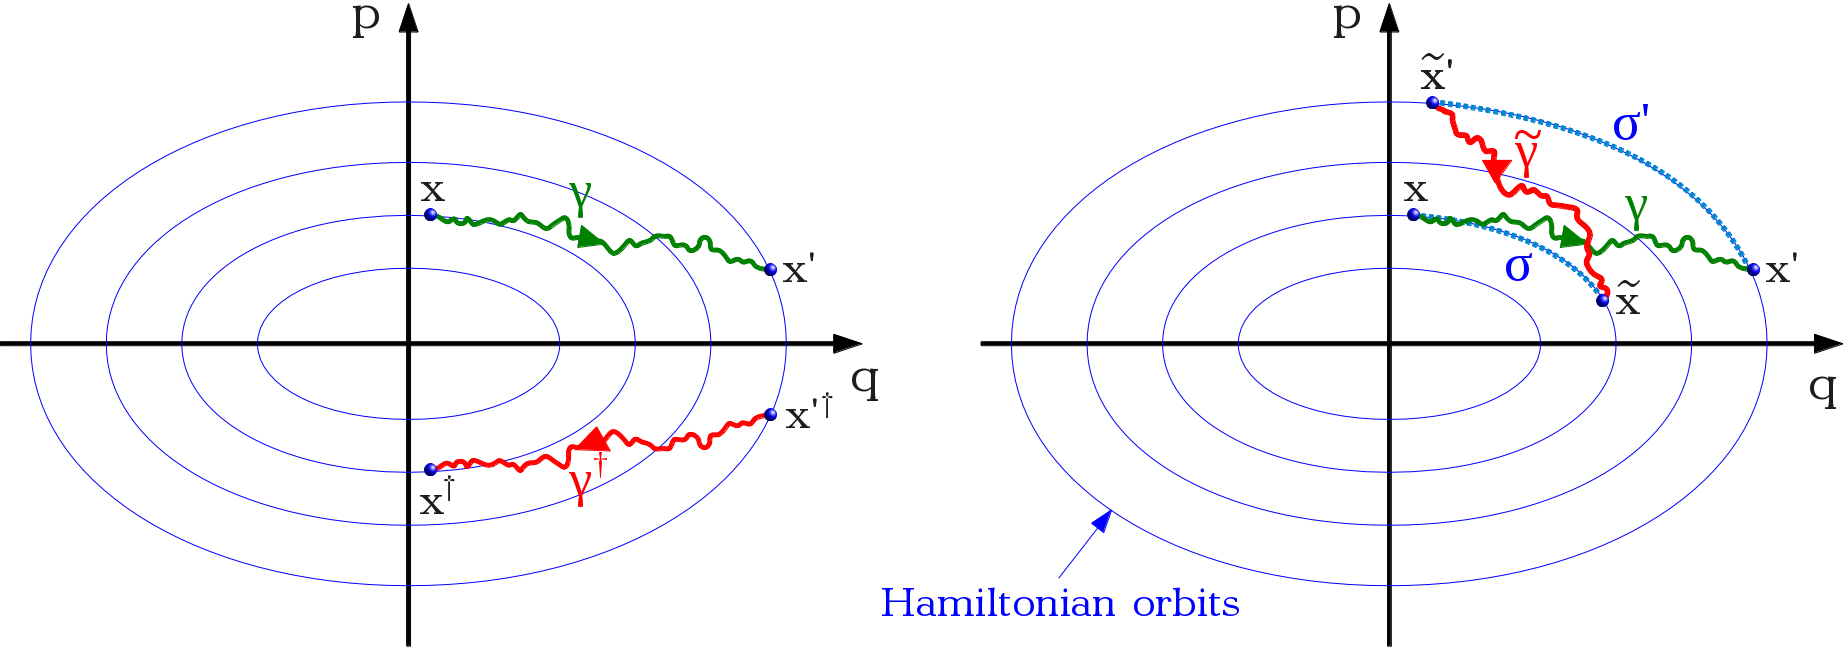
\includegraphics[width=0.9 \linewidth]{figures/trajectories}
	\caption[]{Path construction in the two models. The left side shows SF's approach, which mirrors the forward trajectory \(\gamma\) into a different part of phase space (yielding \(\gamma^\dagger\)), and calculates the ratio of the weights of these two paths. On the right hand side is the flow-based approach, which does not mirror momenta; instead, it traces the Hamiltonian flow in order to reach the start and end points of the conjugate process \(\tilde\gamma\). (Image by Haye Hinrichsen, taken from \cite{flow-paper}.)}
	\label{fig:hf sf}
\end{figure}

%%%%%%%%%%%%%%%%%%%%%%%%%%%%%%%%%%%%%%%%%%%%%%%%%%%%%%%%%%%%%%%%%%%%%%%%%%%%%%
\subsection{Differences between the models}
%%%%%%%%%%%%%%%%%%%%%%%%%%%%%%%%%%%%%%%%%%%%%%%%%%%%%%%%%%%%%%%%%%%%%%%%%%%%%%


At this point may be a good idea to mention figure~\RefFigure{fig:hf sf} again, where the two path constructions (SF and flow) are pictured alongside each other. Important consequences compared to SF's model are as follows:
%
\begin{itemize}
	\item The \HF{} entropy definition is local in phase space: nothing is mirrored into a different part of phase space, and the entire quotient is constrained to an arbitrarily small part of phase space for sufficiently small timespans.
	\item Inside the \HF{} entropy definition, distinction between odd and even variables is necessary, again because of the absence of time or momentum reversal.
	\item No differential entropy is produced for ``transitioning'' onto the same orbit again in the \HF{} case, whereas for \SF{} this is not necessarily so.
\end{itemize}

The second point is particularly important, as it contains what is probably the crucial conceptual difference between \HF{} and \SF{}. For \HF{}, the splitting is done \emph{a priori} with only the equations of motion known, in particular before entropy is even mentioned. On the other hand, in Spinney/Ford's case, reversal of dynamics is hard-wired into the entropy definition itself. In other words, \textbf{the \HF{} approach factors out the reversal of dynamics}.

In order to obtain the conjugate propagator to the original forward process in the \HF{} model, the Hamiltonian part of the equations of motion needs to be known, which allows tracing the Hamiltonian flow back along the deterministic trajectory to reach the starting position of the reverse process, and similarly for the end position. In other words, the equations of motions must be partitioned in two parts, one for the Hamiltonian flow and one for the non-Hamiltonian processes such as dissipation and friction.

The principle behind the algorithm for the separation is inspired by the definition of the Riemann tensor: the system is run in a process that should return to the origin in the end; if it does not, the discrepancy is characteristic for a certain property of that system. In case of the Riemann tensor that discrepancy is the curvature of space, in phase space system it accounts for the non-Hamiltonian parts of the dynamics.

Formally, the most general equations of motion read, with \(x\) = \(q\) or \(p\):
%
\begin{align}
	\dot x &= f_x(q,p) + \Gamma_x(q,p)\xi_x(t)
\end{align}
%
This can be split up in Hamiltonian (\(\dot x_H\)) and non-Hamiltonian (\(\dot x_\Delta\)) parts:
%
\begin{align}
	\dot x &= \dot x_H + \dot x_\Delta
\end{align}
%
To obtain the summands individually, the following algorithm is used:
%
\begin{enumerate}
	\item Calculate \(x(t+\d t/2) \).
	\item Reverse the system's dynamics by substituting \(p \to -p\).
	\item Evolve the for another \(\d t/2\), starting at the previously reached end point.
	\item The end position is \(x(t+\d t)\), from which \(x_\Delta = x(t+\d t) - x(t)\) can be determined.
\end{enumerate}
%
For example, this procedure applied to the underdamped particle discussed in the present work
%
\begin{align*}
	\dot q &= p \\
	\dot p &= -V'(q) - \mu(p)p + \Gamma(p)\xi(t)
\end{align*}
results in
\begin{align*}
	\dot q_H &= p  &  \dot q_\Delta &= 0 \\
	\dot p_H &= -V'(q)  &  \dot p_\Delta &= - \mu(p)p + \Gamma(p)\xi(t) ~.
\end{align*}
This approach is quite general and can be applied to more complicated systems, in which the separation may not be as clear.



%%%%%%%%%%%%%%%%%%%%%%%%%%%%%%%%%%%%%%%%%%%%%%%%%%%%%%%%%%%%%%%%%%%%%%%%%%%%%%
\subsection{Flow-based entropy production of the model}
%%%%%%%%%%%%%%%%%%%%%%%%%%%%%%%%%%%%%%%%%%%%%%%%%%%%%%%%%%%%%%%%%%%%%%%%%%%%%%

This new model can now be applied to the one-dimensional underdamped particle introduced before in section~\RefSection{sec:underdamped-model}. Here, the forward process starts at \(\vec x = (q,p)\) and ends at \(\vec x' = (q',p')\). The conjugate process starts at \(\tilde{\vec x}' = (q'-p'\d t, p'-f(q')\d t)\), which as described before is where tracing back the Hamiltonian orbit through \((q',p')\) for a timespan \(\d t\) reaches; similarly, \(\tilde{\vec x} = (q+p\d t, p+f(q)\d t)\). The entropy thus reads
%
\begin{equation}
	\label{eqn:flow entropy quotient}
	\d\SEnv^\HF(\vec x'|\vec x;\,\d t)
	= \lim_{\varepsilon\to0}
		\frac{
			_\varepsilon G_a(q',p'|q,p;\,\d t)
		}{
			_\varepsilon G_b(q+p\d t, p+f(q)\d t)|q'-p'\d t, p'-f(q')\d t;\,\d t)
		}
\end{equation}
%
where the propagator has no explicit \(t\) dependence, which has therefore been dropped in the notation. The same argument that has been made in the SF case in \RefEqn{eqn:delta-limit} -- namely that in the limit \(\varepsilon\to0\) the location has to behave deterministically, giving a condition on the ambiguity parameters \(a\) and \(b\) -- can be used here to yield
%
\begin{equation}
	\begin{split}
	&(q'-q)-\bigl(p+a(p'-p)\bigr)\d t
	\\=&
	-\Bigl( (q-q')+(p+p')\d t \\
	&\qquad - \bigl( p'-f(q')\d t + b(p-p'+(f(q)+f(q'))\d t)\bigr) \Bigr)
	\end{split}
\end{equation}
%
which holds iff \(a = b = \tfrac12\), as can be shown by expanding the force \(f(q')\) around \(q\) and neglecting terms of \(\Cal O(\d t^3)\). This makes a lot of sense, as it means that the fields are evaluated around the center of each trajectory, which to leading order in time is the same for both processes. This result is much stronger than what is obtained in SF's case, where \(a = b\) is imposed, without giving them a specific value.

Like in the SF chapter before, the entropy production \RefEqn{eqn:flow entropy quotient} can be calculated in this case, yielding \TODO{verify}
%
\begin{equation}\begin{split}
	\label{eqn:hf entropy}
	\d\SEnv^\HF &=
	\frac1{\Gamma^2}\bigl(-2p\mu V'-2\Gamma\Gamma'V'\bigr)\d t
	+ \frac1{\Gamma^2}\bigl(-2p\mu-2\Gamma\Gamma'\bigr)\d p
	\\&\qquad
	+ \frac1{\Gamma^2}\bigl( -p\mu' + 2p\mu \tfrac{\Gamma'}\Gamma - \mu - \Gamma\Gamma'' + \Gamma'^2 \bigr) \d p^2
	\\&\qquad
	+ \Cal O(\d t^2) + \Cal O(\d p^3)
\end{split}\end{equation}
%
where once again the explicit dependencies of the coefficients have been dropped for brevity. This result shows some important differences compared to SF's result \RefEqn{eqn:sf entropy production}:
%
\begin{itemize}
	\item No entropy is produced to leading order in \(\d t\) along the deterministic trajectory \(\d p = -V'(q)\d t\). This is of course a direct result of the construction, which specifically addressed the issue that only switching orbits should yield an entropy contribution.
	\item While the SF result does not include a term proportional to \(\d p^2\), the expression here does.
	\item Applied to a particle in a system with linear friction and additive noise in detailed balance, the expression reduces to the expected textbook result \RefEqn{eqn:classical environmental entropy production}.
	\item The result coincides with the result SF would have gotten, had they not chosen \(a = \tfrac12\) instead of \(0\) in their model -- \RefEqn{eqn:sf entropy production 1/2} is identical to \RefEqn{eqn:hf entropy}! This brings up the question once again as to why they made this specific choice, but as mentioned earlier, this is done without further comment in \cite{sf}.
\end{itemize}






%%%%%%%%%%%%%%%%%%%%%%%%%%%%%%%%%%%%%%%%%%%%%%%%%%%%%%%%%%%%%%%%%%%%%%%%%%%%%%
\section{Towards observable quantities}
%%%%%%%%%%%%%%%%%%%%%%%%%%%%%%%%%%%%%%%%%%%%%%%%%%%%%%%%%%%%%%%%%%%%%%%%%%%%%%

The previously defined quantity \(\d\SEnv(\vec x'|\vec x;\,\d t)\) is a two-point function, yielding the expected entropy production for the transition \(\vec x\to\vec x'\). However, this quantity is not easily accessible by experiment or simulation: while the starting point \(\vec x\) can be set, \(\vec x'\) is much less accessible due to it being statistically distributed over arbitrary phase space regions. The following sections will successively integrate out the unknowns, in order to yield a testable result.


%%%%%%%%%%%%%%%%%%%%%%%%%%%%%%%%%%%%%%%%%%%%%%%%%%%%%%%%%%%%%%%%%%%%%%%%%%%%%%
\subsection{Local entropy production}
%%%%%%%%%%%%%%%%%%%%%%%%%%%%%%%%%%%%%%%%%%%%%%%%%%%%%%%%%%%%%%%%%%%%%%%%%%%%%%

\newcommand\SEnvLoc{\ensuremath{S_\text{env,\,loc}}}

The \emph{local entropy production rate} integrates out the final phase space coordinate:
%
\begin{equation}
	\d\SEnvLoc(\vec x;\,\d t) = \int_\Omega\d\vec x' G_c(\vec x'|\vec x;\,\d t) \d\SEnv(\vec x'|\vec x;\,\d t) + \Cal O(\d t^2)
\end{equation}
%
This describes the expected change in environmental entropy in a short timespan \(\d t\), given an initial location \(\vec x\) in phase space \(\Omega\). Note that the propagator to encode the transition likelihood contains yet another ambiguity parameter in addition to \(a\) and \(b\) implicitly contained in \(\d\SEnv\).

Translated to the present model of a particle in two-dimensional phase space, the equation reads
%
\begin{equation}\begin{split}
	\label{eqn:local entropy 1d}
	\d\SEnvLoc(q,p;\,\d t) &= \inflint\d q'\inflint\d p'\; G_c(q',p'|q,p;\,\d t) \d\SEnv(q',p'|q,p;\,\d t)
	\\&\quad + \Cal O(\d t^2) ~.
\end{split}\end{equation}
%
To calculate its value, first expand the ordinary differential entropy production in terms of differences of its arguments,
%
\begin{equation}
	\label{eqn:dSEnv power expansion}
	\d\SEnv(q',p'|q,p;\,\d t)
	= \sum_{i,j=0}^\infty
	\sigma_{ij}(q,p,\d t)
	(q'-q)^i
	(p'-p)^j
	+ \Cal O(\d t^2)
\end{equation}
%
so that \(\sigma_{ij}\) are the Taylor coefficients of \(\d\SEnv\) in terms of \(q\) and \(p\). Inserting this expansion in \RefEqn{eqn:local entropy 1d} yields
%
\begin{equation}\begin{split}
	\d\SEnvLoc(q,p;\,\d t) &=
	\sum_{i,j=0}^\infty
	\sigma_{ij}(q,p,\d t)
	\\&\qquad
	\times\inflint\d q'
	\inflint\d p'
	\; G_c(q',p'|q,p;\,\d t)
	(q'-q)^i
	(p'-p)^j
	\\&\qquad + \Cal O(\d t^2)
\end{split}\end{equation}
%
where the second line can be identified as the \((i,j)\)-th \((q,p)\) propagator moments respectively,
%
\begin{equation}
	M_{ij,c}(q,p,\d t) = 
	\inflint\d q'
	\inflint\d p'
	\; G_c(q',p'|q,p;\,\d t)
	(q'-q)^i
	(p'-p)^j
\end{equation}
%
which allows rewriting \(\d\SEnvLoc\) as
%
\begin{equation}
	\label{eqn:dSEnvLoc split up}
	\d\SEnvLoc(q,p;\,\d t)
	=
	\sum_{i,j=0}^\infty
	\sigma_{ij}(q,p,\d t)
	M_{ij,c}(q,p,\d t)
	+ \Cal O(\d t^2)
\end{equation}
%
where the expression is split up in two parts that easily combine into the local entropy production: \(\sigma_{ij}\) is obtained via the expansions of the known propagator quotients from the previous section using \RefEqn{eqn:dSEnv power expansion}, and the not yet known propagator moments \(M_{ij,c}\).



In the case of the present model of the underdamped particle \RefEqn{eqn:underdamped sde epsilon}, the propagator moments can be calculated. Due to the length of the intermediate results, this calculation can be found in appendix~\RefSection{sec:fp moments}. The result obtained there is
%
\begin{align}
	M_{00;c} &= 1 + \Cal O(\d t) \\
	M_{01;c} &= (-p\gamma(p) - V'(q)) \d t + \Cal O(\d t^2) \\
	M_{02;c} &= \Gamma(p)^2 \d t + \Cal O(\d t^2) \\
	M_{ij;c} &= \Cal O(\d t^{i+1}) \quad (i,j > 0)
\end{align}
%
These expressions are noteworthy in a couple of ways:
\begin{enumerate}
	\item The ambiguity parameter \(c\) does not appear in terms of leading order, indicating that the propagator moments are independent of said ambiguity at least in the present special case, where the fields are evaluated linearly between start and end points. (Recall that the most general version, introduced in section~\RefSection{sec:general propagator case}, allows evaluation at arbitrary points \(\varphi(\vec x,\vec x')\), whereas here \((1-c)\vec x + c\vec x'\) has been chosen.)
	\item None of the nonzero \(\d q\) moments matter; they all contribute to higher-order in \(\d t\) terms only.
	\item The ad-hoc quantity \(\varepsilon\) of the equations of motion \RefEqn{eqn:underdamped sde epsilon} vanishes naturally in the calculation, once again justifying its previous introduction.
\end{enumerate}

Now \(\d\SEnvLoc\) can be calculated for the Spinney-Ford case with \(a=0\), the Hamiltonian Flow model and therefore also \SF with \(a = \tfrac12\), and remarkably the results are all identical, namely \TODO{verify formula}
%
\begin{equation}\begin{split}
	\d\SEnvLoc(q,p,\d t)
		&=
		\Bigl(-\mu(p) - p \mu'(p) + \frac{2p^2\mu(p)^2}{\Gamma(p)^2} + \frac{4p\mu(p)\Gamma'(p)}{\Gamma(p)} \\
		&\qquad + \Gamma'(p)^2 - \Gamma(p)\Gamma''(p)\Bigr) \, \d t + \Cal O(\d t^2) ~.
\end{split}\end{equation}
%
The terms proportional to \(\d p^2\) in \RefEqn{eqn:hf entropy} compensate the other differences compared to \RefEqn{eqn:sf entropy production} during integration (i.e. multiplication with the propagator moments) by moving them to higher orders of \(\d t\), explaining how different differential entropies can yield the same local entropy production.





%%%%%%%%%%%%%%%%%%%%%%%%%%%%%%%%%%%%%%%%%%%%%%%%%%%%%%%%%%%%%%%%%%%%%%%%%%%%%%
\subsection{Global entropy production}
\label{sec:global entropy production}
%%%%%%%%%%%%%%%%%%%%%%%%%%%%%%%%%%%%%%%%%%%%%%%%%%%%%%%%%%%%%%%%%%%%%%%%%%%%%%

The \emph{global entropy production} once again averages over all positions, to give an expectation value for the short-time environmental entropy production in an ensemble of many (non-interacting) particles. It is obtained from the local entropy production developed just above via
%
\begin{equation}\begin{split}
	\label{eqn:global entropy production}
	\langle\d\SEnv\rangle(t)
	&= \d t \int_\Omega \d\vec x P(\vec x, t)\d\SEnvLoc(\vec x, \d t) \\
	&= \d t \infint\!\!\d q\infint\!\!\d p\, P(q, p, t) \, \d\SEnvLoc(q, p, \d t)
\end{split}\end{equation}
%
where \(P\) is the probability density for being in a certain point of phase space.

For example, take a system in thermal equilibrium. Here, \(\mu(p)\) and \(\Gamma(p)\) are related via the generalized Einstein relation \RefEqn{eqn:einstein}, and \(P(q,p)\) is Boltzmannian. The differential entropy productions then turn out to be
%
\begin{align}
	\d\SEnv^\SF &= -\beta p(\d p + V'(q)\d t) - \frac\beta2\Gamma(p)^2 + \Cal O(\d t^2) + \Cal O(\d p^3) \\
	\d\SEnv^\HF &= -\beta p(\d p + V'(q)\d t) + \Cal O(\d t^2) + \Cal O(\d p^2)
\end{align}
%
which also showcases the previously claimed fact that \SF's result does not vanish along the deterministic trajectory \(\d p = -V'(q)\d t\), while the \HF{} result does. Maybe more importantly even, \SF's result does not reproduce the result previously obtained using only classical thermodynamics in \RefEqn{eqn:classical environmental entropy production}. However, as claimed earlier, the resulting local entropy production is identical for both results,
%
\begin{equation}
	\d\SEnvLoc(q,p,\d t) = \left(
		- \tfrac12\beta\Gamma(p)^2
		+ \tfrac12\beta^2p^2\Gamma(p)^2
		- \beta p\Gamma(p)\Gamma'(p)
		\right)\,\d t
		+ \Cal O(\d t^2) ~.
\end{equation}
%
By integrating this together with the Boltzmann distribution
%
\begin{equation}
	P(q,p) = \frac1Z e^{-\beta\left(\frac{p^2}2-V(q)\right)}
\end{equation}
%
in \RefEqn{eqn:global entropy production}, the global entropy production can be obtained. As the explicit calculation in appendix~\RefSection{sec:global entropy zero} shows, the result is
%
\begin{equation}
	\label{eqn:global entropy 0}
	\forall t. ~ \langle\d\SEnv\rangle(t) = 0
\end{equation}
%
which is what a system obeying detailed balance in thermal equilibrium should obey. This is in agreement with classical thermodynamics again, and the necessity for the previous calculation also hints at why the expression for \(\d\SEnv\) in \RefEqn{eqn:classical environmental entropy production} is not entirely correct: although it assumes \emph{some} properties equilibrium provides, it is a ``thermodynamic'' quantity in terms of \(q\) and \(p\), while classical thermodynamics only deals with averages in which single appearances of location and momentum are meaningless.


%%%%%%%%%%%%%%%%%%%%%%%%%%%%%%%%%%%%%%%%%%%%%%%%%%%%%%%%%%%%%%%%%%%%%%%%%%%%%%
\section{Conclusion}
%%%%%%%%%%%%%%%%%%%%%%%%%%%%%%%%%%%%%%%%%%%%%%%%%%%%%%%%%%%%%%%%%%%%%%%%%%%%%%

Although the initial goal of the presented subject was finding a better definition of entropy production in continuous settings, it turned out that both the new (flow based) and the old (SF, \cite{sf}) approach yield identical results both for the local and the global environmental entropy production in the scenarios presented above. This leads to the conclusion that (two-point) \textbf{short-time environmental entropy production is not a uniquely defined quantity}, and should be regarded as a mathematical intermediate step. However, the flow-based approach seems to be closer to physical intuition, as it does not require a time reversal (which is particularly difficult to map to the real world), its intermediate results vanish along the deterministic trajectory of the system, the distinction between odd and even variables is not necessary, and the propagator ambiguities fall away during the calculation without making further assumptions (which is important to mention because SF and HF models are identical in their two-point entropy production, given the \emph{arbitrary} choice of \(a = \tfrac12\) in the former model).

It is worth noting that the case of a more general system than \RefEqn{eqn:model hamiltonian eqns of motion} has not been investiated, and it is unknown whether both path constructions still agree in this scenario. Furthermore, the SDE of the system has been integrated according to the \Ito{} scheme in order to obtain the FP equation; the consequences of choosing Stratonovich or an arbitrary parameter value for the stochastic integration are also subject to further research.




